\chapter{Preliminary Study} 
\label{Chapter2}
In this chapter, we will proceed through two sections; the first one will define a theoretical background which will be used in this project to solve its problematic. The second one will cover a study of the existing technologies and establish a comparative analysis in order to pick a technical review as a result.
\section{State of the Art}
\subsection{Concepts of Big Data}
\subsubsection{Definitions}
Big Data is a data whose scale, diversity, and complexity require new architecture, techniques, algorithms, and analytics to manage it and extract value and hidden knowledge from it. Traditional databases analytics says what happened and what is happening, however gives the predictive analysis of what is likely to happen in future. Infrastructure requirements of big data are data acquisition, data organization and data analysis \cite{cite16}. \\

The term "Big Data" describes innovative techniques and technologies to capture, store, distribute, manage and analyze
petabyte- or larger-sized datasets with high-velocity and different structures. Big data can be structured, unstructured or semi-structured, resulting in incapability of conventional data management methods \cite{cite17}.\\

Big Data refers to the explosion in the quantity and sometimes quality of available and potentially relevant data, largely the result of recent and unprecedented advancements in data recording and storage technology. In this new and exciting world, sample sizes are no longer measured in number of observations, but rather in megabytes.\\

The most popular definition in the recent years is the "Three V's": volume, velocity , and variety. The concept was first raised by Doug Laney (2001) in his META Group
research note \cite{cite} that describes the characteristics of datasets that cannot be handled by traditional data management tools. With the development of discussion and increasing interest in big data, the "Three V's" have been expanded to "Five V’s": volume, velocity, variety, veracity, value and now it's about multi-V model.
\subsubsection{The 3-V Model}
\label{3vm}
It is generally accepted that big data can be explained according to three V's: Velocity, Variety and Volume.\\

\begin{itemize}
\item \textbf{Velocity:} The phrase velocity represents the data generation speed. Big data velocity deals with the step at which data flows in from sources like business processes, machines, networks and human interaction with things like social media sites, mobile devices etc. The flow of data is massive and continuous. This real time data can help users make valuable decisions. Thus, velocity means analyzing of streaming data.\\

\item \textbf{Variety:} Variety refers to the many sources and types of data, both structured and unstructured. The data is stored in spreadsheets and databases, which comes from different sources. Now data comes in the form of csv files, photos, videos, monitoring devices, PDF, Audio etc. This variety of unstructured data creates problems for storage, mining and analyzing data. In order to defeat this issue, we have to define the data storage system which can analyze variety of data.\\

\item \textbf{Volume:} Big Data implies enormous volumes of data. This data is generated and created for different purposes by machines, networks and human interaction on systems. The volume of data to be analyzed is a huge amount of data. Recently, the data generation sources are augmented and it causes diversity of data such as text, video, audio and databases. In order to process the enormous amount of data, conventional data processing has to be enhanced.\\
\end{itemize}


\subsubsection{From 3-V to multi-V Model}

Big data initially meant the volume, velocity and variety of data that becomes
tricky to analyze by using conventional data processing platforms and techniques. Nowadays, data production sources are improved rapidly, such as sensor networks, high throughput instruments, streaming machines and these environments generate massive amount of data.\\

Nowadays, big data has been playing a crucial role in a variety of environments such as business organization, industry, scientific research, natural resource management, social networking and public administration, and the 3'Vs model is no longer suitable to print the big data features. Therefore, a multi-V model is adopted \cite{cite18}.\\


\begin{itemize}
\item \textbf{Velocity,Variety and Volume:} already defined in section \ref{3vm}.  
\item \textbf{Value:} The value of data indeed represents Big Data. Having continuous amounts of data is not helpful until it can be turned into value. It is essential to understand that doesn't always mean there is value in Big Data. The benefits and costs of analyzing and collecting the big data is more impartment thing when doing big data analytics.
\item \textbf{Veracity:} Veracity represents the data understandability; it
doesn't represent data quality. It is significant that the association should perform data processing to prevent "dirty data" from accumulating in the systems. 
\item \textbf{Validity:} It
is essential to ensure whether the data is precise and accurate for the future use. In
order to take the right decisions in future, the organizations should valid the data
noticeably.
\item \textbf{Variability:} Variability refers to the data consistent and data value.
\item \textbf{Viscosity:} Viscosity is an element of velocity and it represents the latency or lag time in data transmit between the source and destination. 
\item \textbf{Virality:} Virality represents the speed of the data send and receives from various sources.
\item \textbf{Visualization:} Visualization is used symbolize the Big Data in a complete view and determine the hidden values. Visualization is an essential key to making big data an integral part of decision making.
\end{itemize}
\subsubsection{Big Data Analysis}
Techniques for efficiently accessing, analyzing and presenting large amounts of
dynamic, heterogeneous data, with the goal of obtaining new knowledge and facts, play
an increasingly important role in various application domains, such as media, patent
databases, scientific repositories, medical databases etc.\\

Since data is not always moved during the organization step, the analysis may also be done in a distributed environment, where some data will stay where it was
originally stored and be transparently accessed from a data warehouse. The infrastructure required for analyzing big
data must be able to support complex analytics such as statistical analysis and data mining, on a wider variety of
data types stored in diverse systems, scale to extreme data volumes, deliver faster response times driven by changes in
behavior and automate decisions based on analytical models.\\

Most importantly, the infrastructure must be able to integrate analysis on the combination of big data and traditional enterprise data. New insight comes not just from analyzing new data, but from analyzing it within the context of the old to provide new perspectives on old problems. Figure \ref{process} shows the data analysis process.\\

~\\

\begin{figure}[!ht]
\begin{center}
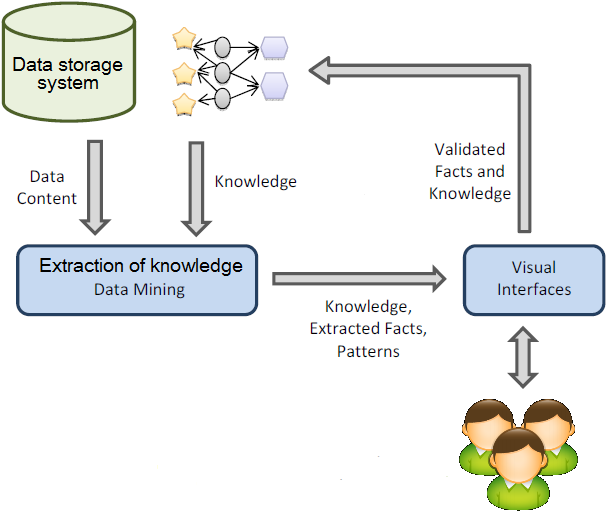
\includegraphics[width=15cm,height=9.8cm]{chapter2/fig9.png}
\end{center}
%légende de l'image
\caption{Data Analysis Process}
\label{process}
\end{figure}
~\\
\subsubsection{Required Infrastructure for Big Data}

Even though the data will be in distributed environment, infrastructure must support to carry out very high transaction volumes and also support flexible data structures. To collect and store data, csv files are often used in big data. Csv files (Comma Separated Values) will not have any fixed schema since it supports high variety of data by capturing all types of data.\\

In the classical term of data warehousing, organizing data is called as data integration. Big data requires good infrastructure, so that processing and manipulating data in the original storage location can be done easily. It must also supports very high throughput to deal with processing steps of large data and handles large variety of data formats like structured format, unstructured format and others. Hadoop is a new technology that allows large data volumes to be organized and processed while keeping the data on the original data storage cluster. Many others distributed frameworks, working over hadoop, are available for data processing. The purpose of this frameworks is to facilitate analytics and improve performance. 

\subsection{Data Mining Tools}
The recent increase of dataset size, in number of records as well as of attributes, has triggered the development of a number of big data platforms as well as parallel data analytics algorithms. At the same time though, it has pushed for the usage of many techniques to extract knowledge from a large set of data. In this section, we will define the main tools used for knowledge extract from data. We have chosen three types of tools which are: dimensionality reduction, clustering and supervised learning algorithms.
\subsubsection{Dimensionality Reduction Procedures}
\label{sectionpca}
Before proceeding with any data analytics task, we need to implement one or more dimensionality reduction techniques. Dimensionality reduction is not only useful to speed up algorithm execution, but actually might help with the final classification or clustering accuracy as well \cite{cite10}.\\ 

\textbf{\normalsize{Principal Component Analysis}}\\

Principal Component Analysis (PCA) is the general name for a technique that uses sophisticated underlying mathematical principles to transforms a number of possibly correlated variables into a smaller number of variables called principal components. The origins of PCA lie in multivariate data analysis, however, it has a wide range of other applications. PCA is one of the most results from applied linear algebra \cite{cite9} and its most common use is to analyse large dataset. It can also be used in de-noising signals, blind source separation and data compression.\\

In general terms, PCA uses a vector space transform to reduce the dimensionality of large data sets. Using mathematical projection, the original data set, which may have involved many variable, can often be interpreted in just a few variables (the principal components). The aim of this section is to explain the theoretical side of PCA.\\

\textbf{\normalsize{The Technical Details of PCA}}\\

As we have mentioned previously, the Principal Component Analysis is above to take a large set of data and identify an optimal new basis in which to re-express the data. \\

The general aim of the PCA method is to find another basis that is a linear combination of the original basis and that re-expresses the data optimally. Let us frame the problem in the following way:\\

Assume that we start with a data set that is represented in terms of an $m \times n$ matrix, $X$ where the $n$ columns are the samples (e.g. observations) and the m rows are the variables. We want to linearly transform this matrix, $X$ into another matrix, $Y$, also of dimension $m \times n$, so that for some $m \times m$ matrix, $P$.\\ 
~\\
\begin{equation*}
\label{eq1}
PX = (Px_{1} Px_{2} \ldots Px_{n})
=
\begin{pmatrix}
    p_{1}x_{1} & p_{1}x_{2}  & \dots  & p_{1}x_{n} \\
    p_{2}x_{1} & p_{2}x_{2}  & \dots  & p_{2}x_{n} \\
    \vdots & \vdots  & \ddots & \vdots \\
    p_{m}x_{1} & p_{m}x_{2}  & \dots  & p_{m}x_{n}
\end{pmatrix}
=
Y
\end{equation*}
~\\ ~\\ 
This equation represents a change of basis. Note that $p_{i},x_{j} \in  \mathbb{R}^{m}$. This tell us that the original data, $X$ is being projected on the column of $P$. Thus, the rows of $P$, $\{ p_{1},p_{2},\ldots,p_{m} \}$ are a new basis for representing the columns of $X$. The rows of P will later become the principal components directions.\\

More details about the principal component analysis in appendix \ref{appendixpca}.


\subsubsection{Clustering}
Clustering is a procedure that divides data into groups which are meaningful, useful, or both. In order to get meaningful group, clusters should capture the natural structure of the data. In some cases, cluster analysis is a useful starting for other purposes, such as data summarization. Other to data analysis, clustering plays an important role in a wide variety of fields: psychology, social sciences, biology and data mining. There have been many applications of cluster analysis to practical problems. \\

Before discussing specific clustering techniques, we provide some necessary background. First, we further define cluster analysis, illustrating why it's difficult. Then, we will explore different techniques that group data.\\

\textbf{\normalsize{Cluster Analysis}}\\

Cluster analysis groups data objects based only on information found in the data that describes the objects and their relationships. The goal is that the objects within a group be similar to one another and different from the objects from the other groups \cite{cite11}. The greater the similarity within a group and the greater the difference between groups, the more distinct the clustering. Figure \ref{fig4} shows three different ways to divide a set of points into clusters. \\
\begin{figure}[H]
\begin{center}
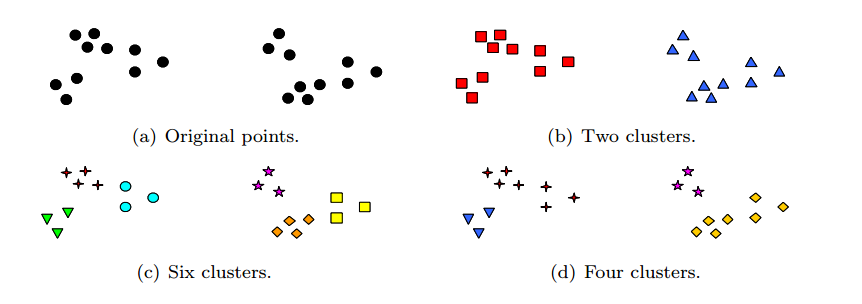
\includegraphics[width=15cm,height=7cm]{chapter2prime/fig1.png}
\end{center}
%légende de l'image
\caption{Different Ways of Clustering the same Set of Points}
\label{fig4}
\end{figure}

\textbf{\normalsize{Approaches to cluster analysis}}\\

There are a number of different methods that can be used to carry out a cluster analysis;
these methods can be classified as follows:
\begin{itemize}
\item Hierarchical methods:
\begin{itemize}
\item Agglomerative methods, in which subjects start in their own separate cluster. The
two "closest" (most similar) clusters are then combined and this is done repeatedly
until all subjects are in one cluster. At the end, the optimum number of clusters is
then chosen out of all cluster solutions.
\item Divisive methods, in which all subjects start in the same cluster and the above strategy is applied in reverse until every subject is in a separate cluster. Agglomerative methods are used more often than divisive methods, so this handout will
concentrate on the former rather than the latter.
\end{itemize}
\item Non-hierarchical methods (often known as k-means clustering methods)
\end{itemize}

\textbf{\normalsize{Data and Measures of Distance}}\\

The data used in cluster analysis can be interval, ordinal or categorical. However, having a mixture of different types of variable will make the analysis more complicated. This is because in cluster analysis we need to have some way of measuring the distance between observations
and the type of measure used will depend on what type of data we have.\\

A number of different measures have been proposed to measure distance for binary and categorical data. For interval data the most common distance measure used is the Euclidean distance. In general, if we have $p$ variables $X_{1},X_{2},\ldots,X_{p},$ measured on a sample of n subjects, the observed data for subject $i$ can be denoted by $x_{i1},x_{i2},\ldots,x_{ip}$ and the observed data for subject $j$ by $x_{j1},x_{j2},\ldots,x_{jp}$. The Euclidean distance between these two subjects in given by:\\
\begin{equation*}
d_{ij}=\sqrt{(x_{i1}-x_{j1})^{2}+(x_{i2}-x_{j2})^{2}+\ldots+(x_{ip}-x_{jp})^{2}}
\end{equation*} 
~\\ ~\\
\textbf{\normalsize{Hierarchical Agglomerative Methods}}\\

Within this approach to cluster analysis there are a number of different methods used to determine which clusters should be joined at each stage \cite{cite19}. The main methods are summarised below \cite{cite20}: 
\begin{itemize}
\item \textbf{Nearest neighbour method (single linkage method):} In this method the distance between two clusters is defined to be the distance between the two closest members, or neighbours. This method is relatively simple but is often criticised because it doesn't take account of cluster structure and can result in a problem called chaining whereby clusters end up being long and straggly. However, it is better than the other methods when the natural clusters are not spherical or elliptical in shape.
 
\item \textbf{Furthest neighbour method (complete linkage method):} In this case the distance between two clusters is defined to be the maximum distance between members — i.e. the distance between the two subjects that are furthest apart. This method tends to produce compact clusters of similar size but, as for the nearest neighbour method, does not take account of cluster structure. It is also quite sensitive to outliers.

\item \textbf{Average (between groups):} linkage method (sometimes referred to as UPGMA) The distance between two clusters is calculated as the average distance between all pairs of subjects in the two clusters. This is considered to be a fairly robust method.

\item \textbf{Centroid method:} Here the centroid (mean value for each variable) of each cluster is calculated and the
distance between centroids is used. Clusters whose centroids are closest together are merged. This method is also fairly robust.

\item \textbf{Ward's method:} In this method all possible pairs of clusters are combined and the sum of the squared
distances within each cluster is calculated. This is then summed over all clusters. The combination that gives the lowest sum of squares is chosen. This method tends to produce clusters of approximately equal size, which is not always desirable. It is also quite sensitive to outliers. Despite this, it is one of the most popular methods, along with the average linkage method.

\end{itemize}

It is generally a good idea to try two or three of the above methods. If the methods agree reasonably well then the results will be that much more believable.\\

\textbf{\normalsize{K-means Clustering}}\\

k-means clustering is a method of vector quantization, that is popular for cluster analysis in data mining. k-means clustering aims to partition n observations into k clusters in which each observation belongs to the cluster with the nearest mean, serving as a prototype of the cluster. This results in a partitioning of the data space into Voronoi cells.
K-means clustering is a method commonly used to automatically partition a data set into k groups. It proceeds by selecting k initial cluster centers and then iteratively refining them as follows:
\begin{itemize}
\item Each instance $d_i$ is assigned to its closest cluster center.
\item Each cluster center $C_j$ is updated to be the mean of its constituent instances.
\end{itemize}

The algorithm converges when there is no further change in assignment of instances to clusters.
\newpage
\subsubsection{Supervised Learning}
Supervised Learning is simply a formalization of the idea of learning from examples. In supervised learning, the learner is provided with two sets of data, a training set and a test set. The idea is for the learner to learn from a set of labeled examples in the training set so that it can identify unlabeled exemples in the test set with the highest possible accuracy \cite{cite21}.\\

A supervised learning algorithm analyzes the training data and produces an inferred function, which is called a classifier, if the output is discrete, or a regression function, if the output is continuous. \\

\textbf{\normalsize{Linear Regression}}\\

Linear regression is an approach for modelling the relationship between a scalar dependent variable y and one or more explanatory (independent) variables. It is used for correlation analysis and tries to come up with the best model that fits the values of independent variables. \\

Linear regression is used for predicting the value of dependent variable with as little error as possible rather than predicting the class label. In order to do this, it needs to learn the correlated features by calculating the linear coefficients of the independent variables according to the following formula:\\ 

\begin{equation*}
y_{i}=\beta_{1}x_{i1}+\ldots+\beta_{p}x_{ip}+\varepsilon_{i}=X_{i}^{T}\beta+\varepsilon_{i}, i=1,\ldots,n
\end{equation*}

As seen from the regression formula, a linear regression model assumes that the relationship between the dependent variable $y_{i}$ and the vector of regressors $x_i$ is linear. Error variable $\varepsilon_{i}$ is an unobserved random variable that adds noise to the linear relationship between the dependent variable and regressors.\\

After coefficients are calculated through learning and model is created that will produce the red line in figure \ref{Regression}, this model will be used to predict the value of the dependent variable based on the input values of the independent variables.\\
\begin{figure}[H]
\begin{center}
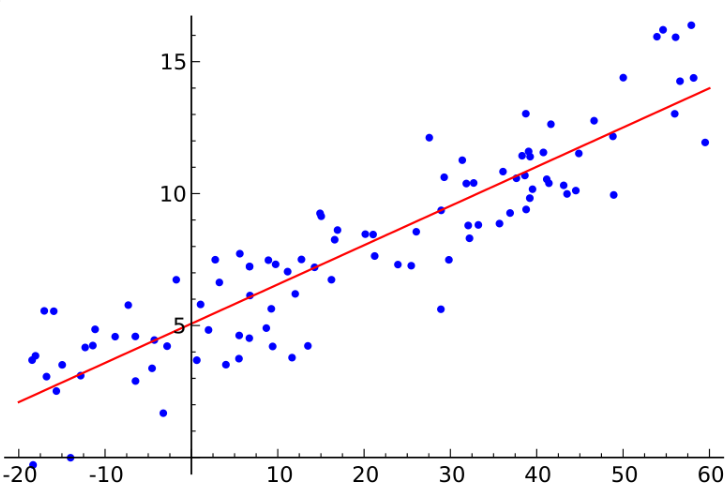
\includegraphics[width=14.5cm,height=7.5cm]{chapter2prime/lr.png}
\end{center}
%légende de l'image
\caption{Linear Regression Representation}
\label{Regression}
\end{figure}


\textbf{Evaluation Metrics for Model Correctness:} Calculation of residuals is crucial for assessing the correctness of the regression model. Residuals are the differences between the observed and predicted values by the model. Using these residual values, evaluation metrics can be calculated:\\

The sum of squared residuals (SSE):
\begin{align*}
SSE&=\Sigma(y_{i}-\widehat{y_{i}})^2\\
R^{2}_{a}&=\dfrac{[(n-1)R^{2}-k]}{[n-(k+1)]}\\
\hat{\sigma}^2 &=\dfrac{SSE}{n-(k+1)}=MSE
\end{align*}

The sum of squared total residuals (SST):
\begin{align*}
SST&=\Sigma(y_{i}-\bar{y}_{0})^{2} \\
f&=\dfrac{R^2/k}{(1-R^{2})/[n-(k+1)]} \\R^2 &= 1-\dfrac{SSE}{SST}
\end{align*}


\textbf{\normalsize{Classifications}}\\

Classification is an instance of supervised learning \cite{cite22}. It is the problem of identifying to which of a set of categories a new observation belongs, on the basis of a training set of data containing observations  whose category membership is known. Classification is an example of pattern recognition. Classification is an example of the more general problem of pattern recognition, which is the assignment of some sort of output value to a given input value. Figure \ref{classification} shows the classification process.\\
~\\ ~\\
\begin{figure}[H]
\begin{center}
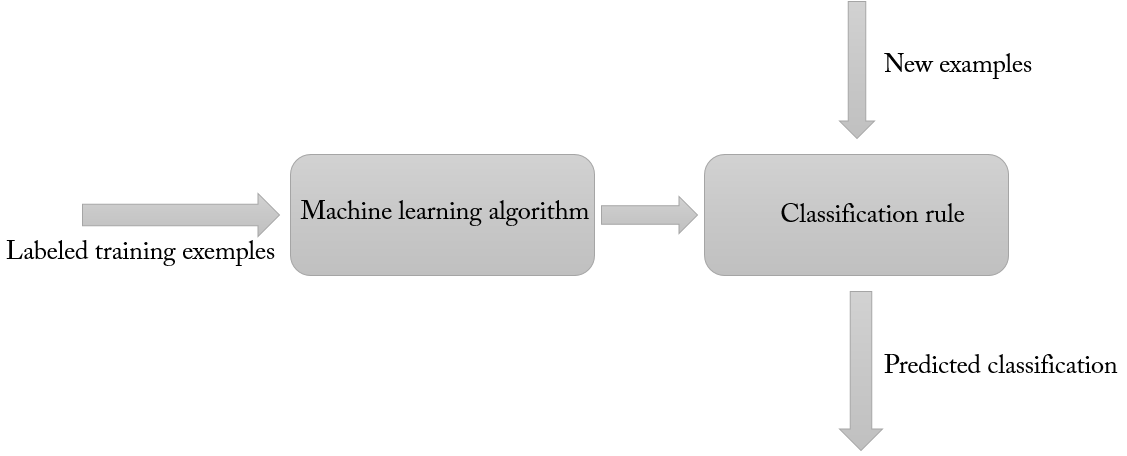
\includegraphics[width=16.5cm,height=7.5cm]{chapter2prime/fig3.png}
\end{center}
%légende de l'image
\caption{Classification Process}
\label{classification}
\end{figure}
\newpage
Example of classification algorithms include:
\begin{itemize}
\item Linear classifiers
\begin{itemize}
\item Fisher's linear discriminant
\item Logistic regression
\item Naive Bayes classifier
\item Perceptron
\end{itemize}
\item Support vector machines
\item Quadratic classifiers
\item Kernel estimation
\begin{itemize}
\item k-nearest neighbor
\end{itemize}
\item Decision trees
\begin{itemize}
\item Random forests 
\end{itemize}
\item Neural networks
\item Learning vector quantization
\end{itemize}

A review of data analysis techniques is represented in figure \ref{analysis}.
\begin{figure}[H]
\begin{center}
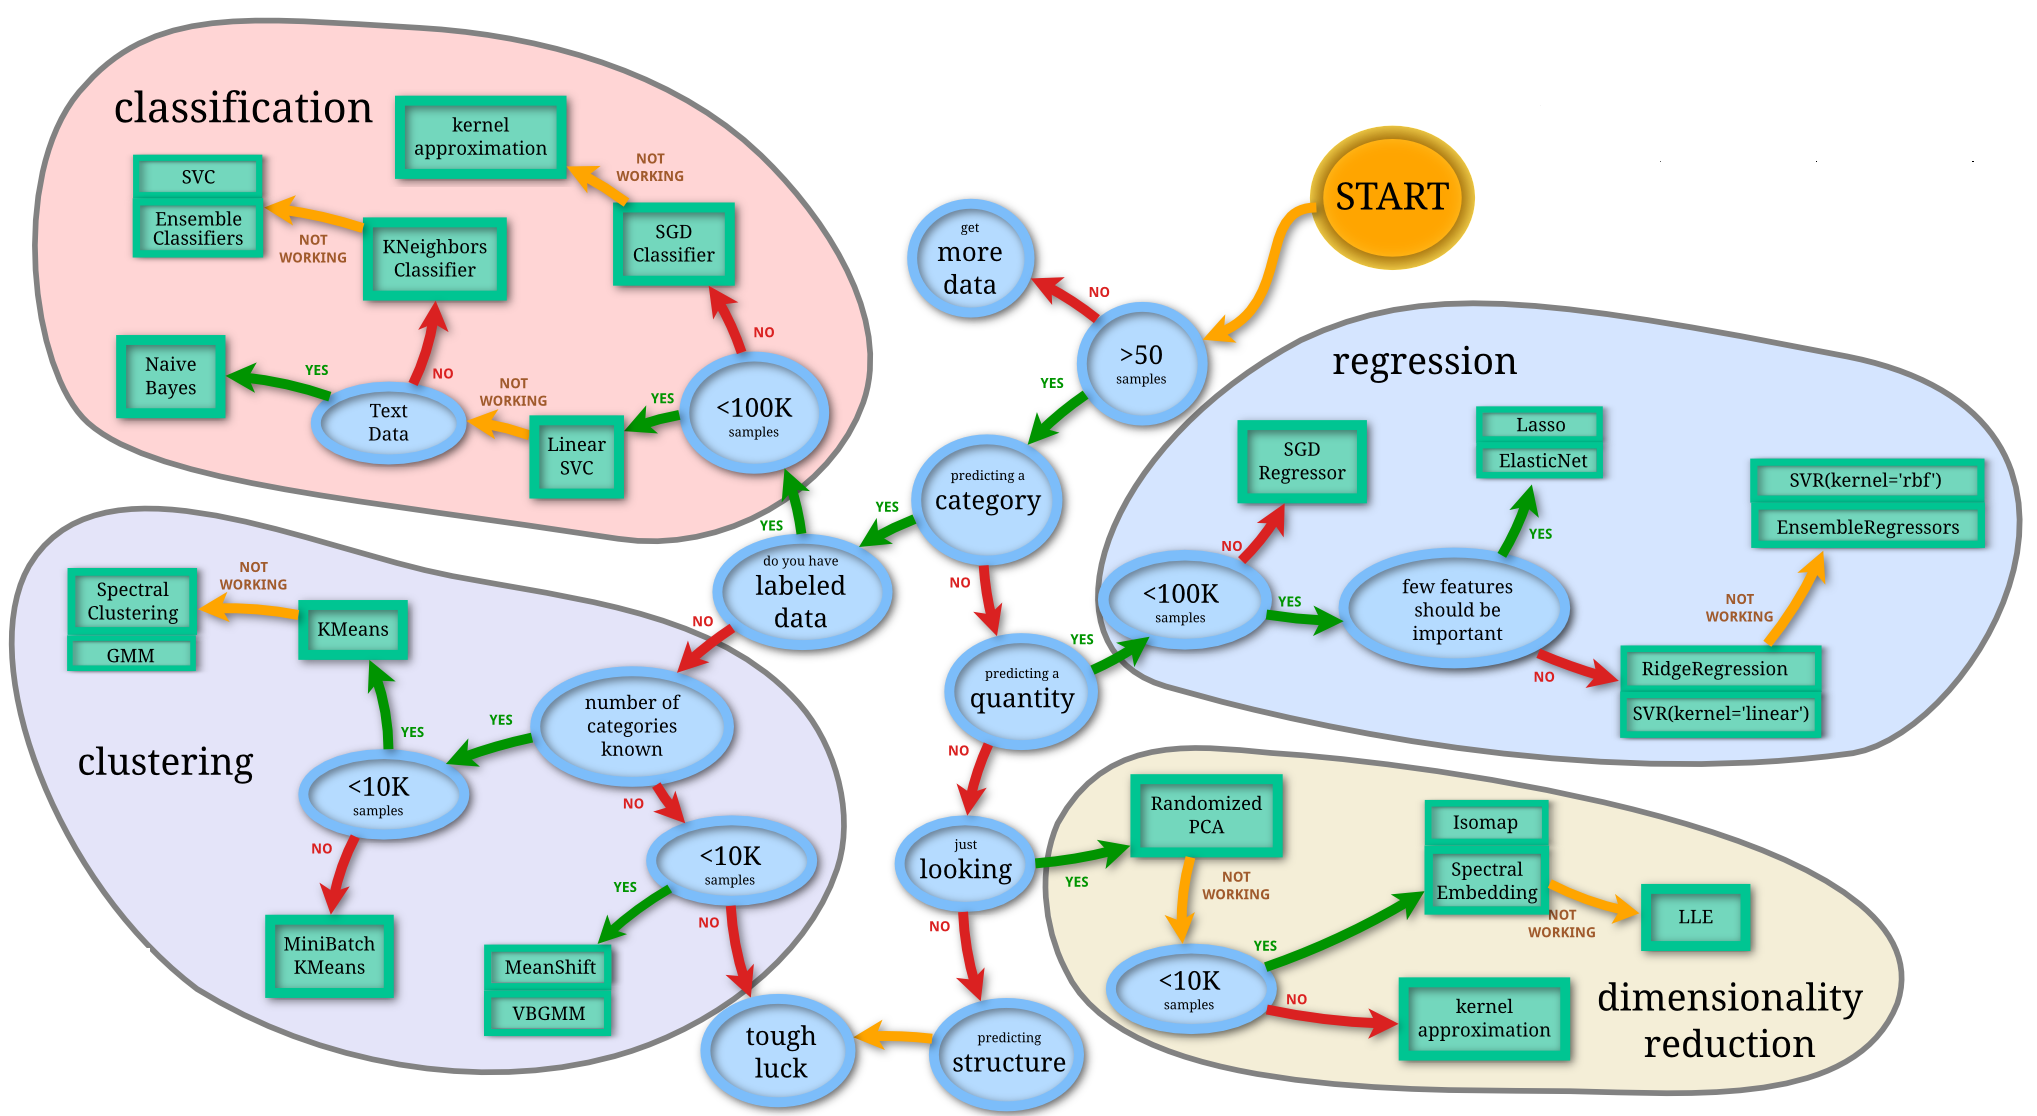
\includegraphics[width=17cm,height=12.2cm]{chapter2prime/fig2.png}
\end{center}
%légende de l'image
\caption{Data Analysis Techniques}
\label{analysis}
\end{figure}


\subsubsection{Data Representation}
Using visual representations to present data makes it easier to understand. Bar graphs, pie charts, line graphs, and histograms are an excellent way to illustrate data processing results. This section includes concepts and definitions, types of graphs
and charts \cite{cite12}.\\
~\\~\\
\textbf{\normalsize{Major Concepts and Definitions}}\\

Graphs and charts condense large amounts of information into easy-to-understand formats that clearly and effectively communicate important points. In selecting how best to present data,we have to think about the purpose of our graph or chart and what we want to present, then decide which variables we want to include and whether they should be expressed as frequencies, percentages, or categories.\\

When we decide what kind of graph or chart best illustrates our data, we should consider what type of data we are working with. Categorical data are grouped into non-overlapping categories (such as grade, race, and yes or no responses). Bar graphs, line graphs, and pie charts are useful for displaying categorical data. Continuous data are measured on a scale or continuum (such as weight or test scores). Histograms are useful for displaying continuous data.\\
~\\
\textbf{\normalsize{Types of Graphs and Charts}}\\

The main types of graphs, that can reduce complexity of unstructured data by transforming it into understandable form, are:\\
\begin{itemize}
\item \textbf{A bar graph} is composed of discrete bars  that represent different categories of data. The length or height of the bar is equal to the quantity within that category of data. Bar graphs are best used to compare values across categories.\\
\item \textbf{A pie chart} is a circular chart used to compare parts of the whole. It is divided into sectors that are equal in size to the quantity represented.\\
\item \textbf{A line graph} displays the relationship between two types of information, such as number of school personnel trained by year. They are useful in illustrating trends over time.\\
\item \textbf{A histogram} has connected bars that display the frequency or proportion of cases that fall within defined intervals or columns. The bars on the histogram can be of varying width and typically display continuous data.\\ 
\end{itemize}



%%%%%%%%%%%stop here
\newpage
\section{Study of The Existing}
In this section, we will establish a comparative study between already existing tools and take by the end which are the best tools that can be adopted in our project. 
\subsection{Existing Tools}
\subsubsection{Relational Database Management System}

\textbf{\normalsize{Drizzle:}}\\

Drizzle is a MySQL fork with a pluggable micro-kernel and with an emphasis of performance over compatibility. Like MySQL, Drizzle had a client/server architecture and uses SQL as its primary command language.

\begin{table}[H]
\caption{Drizzle Advantages and Disadvantages}
\begin{center}
\begin{tabularx}{17cm}{ |p{8.5cm}|X| } 
 \hline
 \textbf{Advantages} & \textbf{Disadvantages } \\ \hline
 $\bullet$ Better performance in modern machines \newline $\bullet$ Can run more than 4 hardware threads at once \newline $\bullet$ Drizzle can operate dynamic multi-statement SQL. Via the key word CONCURRENT, it can operate these statements in parallel. &  $\bullet$ Relational databases are not a suitable solution for large scale data management and analysis processing. \\ \hline

\end{tabularx}
\end{center}
\end{table}
\subsubsection{Non Relational Database Management System}
\textbf{\normalsize{MongoDB:}}\\

MongoDB is an open source NoSQL database that uses a document-oriented data model. Instead of using tables and rows as in relational databases, MongoDB is built on an architecture of collection and documents. Documents comprises sets of key-value pairs and are the basic unit of data in MongoDB. Collection contains sets of documents and function as the equivalent of relational database tables.\\



\begin{table}[H]
\caption{MongoDB Advantages and Disadvantages}
\begin{center}
\begin{tabularx}{17cm}{ |p{8.5cm}|X| } 
 \hline
 \textbf{Advantages} & \textbf{Disadvantages } \\ \hline
 $\bullet$ Horizontal scalability \newline $\bullet$ If the primary server goes down, the secondary server become the primary server without any human intervention\newline $\bullet$ It supports the common authentication mechanisms, such as LDAP, AD, and certificates. Users can connect to MongoDB over SSL and the data can be encrypted. \newline $\bullet$ MongoDB can be a cost effective solution because improves flexibility and reduces cost on hardware and storage. &  $\bullet$ No support transaction \newline $\bullet$ No join \newline $\bullet$ Memory limitation \\ \hline

\end{tabularx}
\end{center}
\end{table}
\newpage
\textbf{\normalsize{Cassandra:}}\\

Apache Cassandra is a free and open-source distributed NoSQL database management system designed to handle large amounts of data across many commodity servers, providing high availability with no single point of failure. Cassandra offers robust support for clusters spanning multiple data centers, with asynchronous masterless replication allowing low latency operations for all clients.\\



\begin{table}[H]
\caption{Cassandra Advantages and Disadvantages}
\begin{center}
\begin{tabularx}{17cm}{ |p{8.5cm}|X| } 
 \hline
 \textbf{Advantages} & \textbf{Disadvantages}  \\ \hline
  $\bullet$ Write speed \newline $\bullet$ Tunable consistency: Cassandra enables, on query-by-query basis, to decide how to handle potential issues. \newline $\bullet$ JVM based that means that Cassandra can easily integrate with other JVM based applications. \newline $\bullet$ CQL: is a familiar way of querying Cassandra, making the transition from an SQL based RDBMS to Cassandra less jarring. & $\bullet$ The Cassandra data storage layer is a key-value storage system. So, data should be modeled around the queries we want to surface, rather than around the structure of the data itself \newline $\bullet$ No Aggregations \newline $\bullet$ Unpredictable Performance due to no user-scheduled tasks \newline $\bullet$ Memory management is done by the language itself, not the application.  \\ \hline

\end{tabularx}
\end{center}
\end{table}
\subsubsection{Data Warehouse}
\textbf{\normalsize{Hive:}}\\

Hive is a data warehouse infrastructure build on Hadoop for providing data summarization query, and analysis. Hive gives an SQL-like interface to query data stored in various databases and file systems that integrate with Hadoop Traditional SQL queries must be implemented in the MapReduce java API to execute SQL applications and queries over distributed data.

\begin{table}[H]
\caption{Hive Advantages and Disadvantages}
\begin{center}
\begin{tabularx}{17cm}{ |p{8.5cm}|X| } 
 \hline
 \textbf{Advantages} & \textbf{Disadvantages}  \\ \hline
 $\bullet$ HIVE is very similar to SQL \newline $\bullet$ Data to be analyzed is stored in HDFS which provides all features like scalability, redundancy etc and SQL like query over data in Hadoop. \newline $\bullet$ Very useful for people who are not from Programming back ground (instead of writing 100 lines of MapReduce/Java program, same requirement can be done using 4 lines of a hive query) \newline $\bullet$ Used to handle structured data & $\bullet$ No real time access to data \newline $\bullet$ Updating data is complicated: \newline - Mainly because of using HDFS \newline - Can overwrite partitions \newline - Can add records \newline $\bullet$ High latency \newline $\bullet$ Slow  \\ \hline

\end{tabularx}
\end{center}
\end{table}

\subsubsection{Data Processing Frameworks}
\textbf{\normalsize{Hadoop:}}\\

Apache Hadoop is an open-source software framework used for distributed storage and processing of big data sets using the MapReduce programming model. It consists of computer clusters built from commodity hardware. All the modules in Hadoop are designed with a fundamental assumption that hardware failures are common occurrences and should be automatically handled by the framework.\\

The core of Apache Hadoop consists of a storage part, known as Hadoop Distributed File System (HDFS), and a processing part which is a MapReduce programming model. Hadoop splits files into large blocks and distributes them across nodes in a cluster. It then transfers packaged code into nodes to process the data in parallel. This approach takes advantage of data locality where nodes manipulate the data they have access to. This allows the dataset to be processed faster and more efficiently than it would be in a more conventional supercomputer architecture that relies on a parallel file system where computation and data are distributed via high-speed networking.\\

The base Apache Hadoop framework is composed of the following modules:
\begin{itemize}
\item Hadoop Common: contains libraries and utilities needed by other Hadoop modules
\item Hadoop Distributed File System (HDFS): is a distributed file-system that stores data on commodity machines, providing very high aggregate bandwidth across the cluster
\item Hadoop YARN: a resource-management platform responsible for managing computing resources in clusters and using them for scheduling of users' applications
\item Hadoop MapReduce: an implementation of the MapReduce programming model for large scale data processing
\end{itemize}




\begin{table}[H]
\caption{Hadoop Advantages and Disadvantages}
\begin{center}
\begin{tabularx}{17cm}{ |p{8.5cm}|X| } 
 \hline
\textbf{Advantages} & \textbf{Disadvantages } \\ \hline
 $\bullet$ Scalable: it can store and distribute very large data sets across hundreds of inexpensive severs that operate in parallel \newline $\bullet$ Cost effective \newline $\bullet$ Flexible \newline $\bullet$ Fast \newline $\bullet$ Resilient to failure & $\bullet$ Security Concerns \newline $\bullet$ Vulnerable by nature \newline $\bullet$ Not fit for small data \newline $\bullet$ Potential Stability Issues \newline $\bullet$ General Limitation  \\ \hline

\end{tabularx}
\end{center}
\end{table}
\textbf{\normalsize{Blobseer:}}\\

BlobSeer is a large-scale distributed storage service that addresses advanced data management requirements resulting from ever-increasing data sizes. It is centered around the idea of leveraging versioning for concurrent manipulation of binary large objects in order to efficiently exploit data-level parallelism and sustain a high throughput despite massively parallel data access.\\



\begin{table}[H]
\caption{Blobseer Advantages and Disadvantages}
\begin{center}
\begin{tabularx}{17cm}{ |p{8.5cm}|X| } 
 \hline
 \textbf{Advantages} & \textbf{Disadvantages}  \\ \hline
 $\bullet$ A single process that writes on a large file (> 20 GB) \newline $\bullet$ Processes that read the same parts of a single file at the same time \newline $\bullet$ Processes that write in the same large file \newline $\bullet$ Fine-grained write access \newline $\bullet$ Good horizontal scalability \newline $\bullet$ Applicable to Hadoop Map/Reduce applications (it comes with a HDFS compatibility layer) & $\bullet$ The version manager is a single point of failure, and hot spot (in the critical path for both reads or writes) \newline $\bullet$ Metadata distribution in a distributed tree may cause high latency as the size of the tree grows \newline $\bullet$ No eviction for old version, causing decreasing performance over time  \\ \hline

\end{tabularx}
\end{center}
\end{table}

\textbf{\normalsize{Spark Apache:}}\\

Apache Spark is a fast and general engine for large-scale data processing. Spark powers aa stack of libraries including SQL and Data Frames, MLlib for machine learning, GraphX, and spark Streaming.\\

Spark extends its predecessors with in-memory processing. Its Resilient Distributed Dataset (RDD) abstraction enables developers to materialize any point in a processing pipeline into memory across the cluster, meaning that future steps that want to deal with the same data set need not recompute it overload it from disk.\\

Sparks runs on Hadoop, Mesos, standalone, or in the cloud. It can access diverse data sources including HDFS, Cassandra and HBase.

\begin{table}[H]
\caption{Spark Advantages and Disadvantages}
\begin{center}
\begin{tabularx}{17cm}{ |p{8.5cm}|X| } 
 \hline
 \textbf{Advantages} & \textbf{Disadvantages}  \\ \hline
 $\bullet$ Faster batch processing than MapReduce. Spark executes batch-processing jobs 10 to 100 times faster than MapReduce \newline $\bullet$ Spark comes with GraphX, a distributed graph system \newline $\bullet$ Spark is ideal for iterative processing, interactive processing and event stream processing \newline $\bullet$ Spark can run on Hadoop alongside other tools in the Hadoop ecosystem including Hive & $\bullet$ Spark is still working out bugs as it matures.\\ \hline

\end{tabularx}
\end{center}
\end{table}
\subsection{Technical Specification}
Spark Apache, as a Bigdata provessing tool, provides mainly four API in four different programming languages which are: Java, Scala, R and Python. Java is a programming language that uses JVM (Java Virtual Machine) which make it no suitable for processing a large scale of data. R is interpreted programming language oriented to Data Science users, but it is made for executing some specified operations and not making a whole application or service that can be used through other applications. So, we have to choose between Scala and Python programming language.\\

Table \ref{cmp} is an established comparison between Python and Scala as two programming languages applied on Apche Spark. 
~\\ ~\\ ~\\
\begin{table}[H]
\caption{Scala Vs. Python on Apache Spark}
\begin{center}
\begin{tabularx}{17cm}{ |p{2.8cm}|X|X| } 
 \hline
 \textbf{Criteria} & \textbf{Scala} & \textbf{Python} \\ \hline
  Learning curve & Scala’s syntax makes it difficult to master & Python is comparatively easier to learn because of its syntax and standard libraries.\\ \hline
  Concurrence & Scala allows developers to write efficient, readable and maintainable services without dangling the program code into an unreadable cobweb of call-backs. & Python does support heavyweight process forking using uwsgi but it does not support true multithreading.\newline
(When using Python for Spark, irrespective of the number of threads the process has only one CPU is active at a time for a Python process. This helps get around with one process per CPU core but the downfall to this is, that whenever a new code is to be deployed, more processes need to restart and it also requires additional memory overhead. Scala is more efficient and easy to work with in these aspects.)\\ \hline
  Type safety & Statically typed language (Scala is a statically typed language through it appears like a dynamically typed language because of the classy type inference mechanism. Being a statically typed language, Scala still provides the compiler to catch compiler to catch compile time errors) & Dynamically typed language (Developers often face difficulties after modifying Python program as it creates more bugs than fixing the older ones.\\ \hline
  Performance & Scala is faster when there are less number of cores. As the number of cores increases, the performance advantage of Scala starts to dwindle) & For a big number of cores, Python is faster than Scala and present a better execution time \\ \hline
  Ease of use & Verbose language & Less verbose and easier to use than Scala\\ \hline
  Advanced \newline features & Has several existential types, macros and implicits but lacks good visualization and local data transformations.
(The arcane syntax of Scala might make it difficult to experiment with the advanced features which might be incomprehensible to the developers. / Scala lacks good visualization and local data transformations.) & Has several libraries for machine Learning and Natural language processing.
(Python has sufficient data science tools and libraries for machine learning, SparkMLlib / Python Spark streaming support is not advanced and mature like Scala)\\ \hline
  Documentation/\newline community &Scala belongs to the tier1 (classified by \#tags in stack overflow and GitHub) & Python belongs also to the tier1. If we consider documentation of the machine learning and statistics frameworks, the Python data science community is more mature.\\ \hline
\end{tabularx}
\end{center}
\label{cmp}
\end{table}
\newpage
\section{Technical Review}
As we have, in our case, a huge amount of unstructured data, the most suitable framework to process advanced and complex analytical algorithms on that data is \textbf{Spark Apache}, as it provides a rich libraries and features that can be adapted to our work. Spark Apache is well performed with \textbf{Python programming language}. In fact, Python provides a variety of tools to present data structure and a plenty of libraries for data mining and data science. Data storage needs also a well performing tool to maintain a large scale of data well maintained for data processing and data-keep-in-security, \textbf{Hadoop Distributed File System (HDFS)} is file system that matches perfectly with Spark Apache. 
 

\section*{Conclusion} 

Throughout this chapter, we explained some theoretical concepts that are essential to understand what follows. We have also established an existing study on which we compared the already existing tools for manufacturing Bigdata. Based on the studied solutions, we will be able to set our project requirements. But before going through this step, we have to define how the chosen tools work. That is the purpose of the coming chapter.